

\section{Distancia Entre Algoritmos}
Utilizar lo visto en clase para implementar un algoritmo en python que permita calcular la distancia entre dos documentos. Los documentos estarán guardados en archivos .txt y se leerán como parametros de ejecución del programa (tarea1.py documento1.txt documento2.txt). El programa debe retornar la distancia entre los dos documentos medida en radianes. Trate de hacer una implementación que sea de rápida ejecución, para ello deberá investigar los tiempos teóricos de ejecución de las funciones a utlizar dentro de python.

\section{Heaps}
Dado el arreglo de números enteros \textit{nums} se eligen dos índices diferentes \textit{i} y \textit{j} del arreglo. Se debe retornar el valor máximo de \textit{nums[i]-1*(nums[j]-1)}.

\textbf{Ejemplo:}

\begin{description}
	\item[Entrada: ] nums $=\, [3,4,5,2]$
	\item[Salida: ] $12$
	\item[Explicación: ] Si se eligen los índices $i=1$ y $j=2$ se obtendrá el producto más grande, a saber, $(4-1)*(5-1)=12$.
	\item[Restricciones: ]
	\begin{itemize}
		\item $2\leq$ nums.length $\leq 500$
		\item $1\leq $ nums[i] $\leq 10^3$
	\end{itemize}
\end{description}
\href{https://leetcode.com/problems/maximum-product-of-two-elements-in-an-array/discuss/?currentPage=1&orderBy=hot&query=}{Fuente}
%\begin{lstlisting}
%	
%\end{lstlisting}


\section{Algoritmo Karp$-$Rabin}

Leer el artículo \href{https://www.geeksforgeeks.org/rabin-karp-algorithm-for-pattern-searching/}{Geeks for Geeks} y ver el vídeo \href{https://www.youtube.com/watch?v=qQ8vS2btsxI}{Youtube}. Con ello elaborar un documento en LaTeX con tres bullet para el artículo y tres para el vídeo de tres o cuatro lineas que describa las ideas centrales de cada uno.

\section{Tarea 4}
Dada el nodo \textit{raíz} de un árbol de búsqueda binaria y dos enteros \textit{low} y \textit{high}, retornar el valor de la suma de todos los valores de todos los nodos cuyos valores, inclusive, están en el rango \textit{[low, high]}.

\textbf{Ejemplo 1:}

\begin{figure}[H]
	\centering
	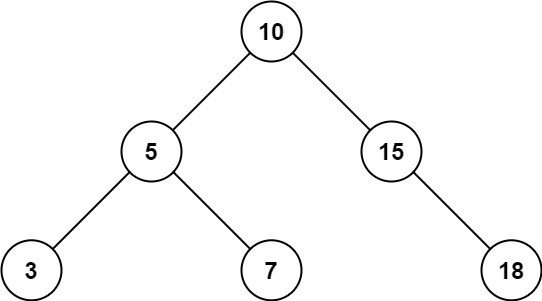
\includegraphics[scale=0.5]{bst1.jpg}
	\label{f1}
\end{figure}

\begin{description}
	\item[Entrada: ] root $=\, [10,5,15,3,7,null,18]$, low = 7, high = 15
	\item[Salida: ] $32$
	\item[Explicación: ] Nodes 7, 10 and 15 are in the range $[7,15]$. $7+10+15=32$.
\end{description}



\textbf{Ejemplo 2:}

\begin{figure}[H]
	\centering
	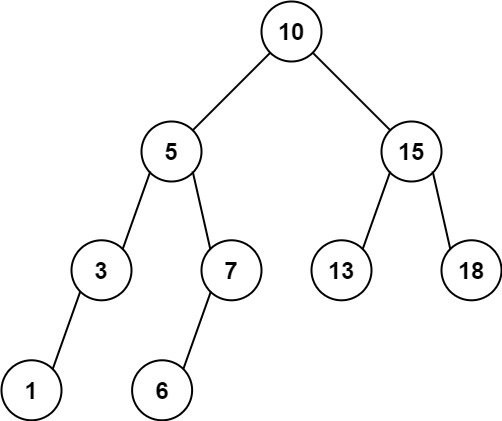
\includegraphics[scale=0.5]{bst2.jpg}
	\label{f2}
\end{figure}

\begin{description}
	\item[Entrada: ] root $=\, [10,5,15,3,7,13,18,1,null,6]$, low = 6, high = 10
	\item[Salida: ] $23$
	\item[Explicación: ] Nodes 6, 7, and 10 are in the range $[6, 10]$. $6 + 7 + 10 = 23$.
\end{description}

\textbf{Restricciones:}
\begin{itemize}
	\item El número de nodos en el árbol está en el rango $[1, 2 * 10^4]$.
	\item $1\leq Node.val \leq 10^5$
	\item $1 \leq low \leq high \leq 10^5$
	\item Todos los Node.val son únicos \textbf{unique}.
\end{itemize}

\href{https://leetcode.com/problems/range-sum-of-bst/}{LeetCode}




\section{Hoja de Trabajo}
Ver \href{https://www.youtube.com/watch?v=pVfj6mxhdMw}{Youtube} y \href{https://www.youtube.com/watch?v=obWXjtg0L64}{Youtube 2}. Con ello elaborar un documento en LaTeX con tres bullet para cada video, de tres o cuatro lineas que describa las ideas centrales de cada uno.




\section{Práctica 1}
Inscribirse al curso \href{https://leetcode.com/study-plan/}{Study Plan} al plan de Estructuras de Datos I. El programa consiste en ir resolviendo problemas diariamente. Su práctica consiste en irlos resolviendo, ingresando sus soluciones en el LeetCode y además crear un repositorio de soluciones en GitHub que deberán subir. Además, deberán elegir uno de los problemas a la semana y hacer su análisis algoritmico (uno diferente cada uno, se ponen de acuerdo entre ustedes cual van a elegir para que no tengamos repetidos), poniendo el código en un documento LaTeX y su respectivo análisis. Al finalizar, deberán presentar el documento PDF y código LaTeX, en el documento PDF deberán poner el enlace al repositorio de Github.




\section{Práctica 2}

Resolver los problems sets 5 y 6 que se encuentran en \href{https://ocw.mit.edu/courses/electrical-engineering-and-computer-science/6-006-introduction-to-algorithms-fall-2011/assignments/}{MIT}. Entregar un solo PDF hecho en  LaTeX para estos dos problems sets. En los casos en que pida escribir pseudocódigo, ustedes deberán escribirlo en python. Al final del reporte, deben consignar el repositorio github donde se pueden ver los códigos.




\section{Práctica 3}

Inscribirse a los cursos \href{https://leetcode.com/study-plan/}{Study Plan} a los planes Algorithms I y II . El programa consiste en ir resolviendo problemas diariamente. Su práctica consiste en irlos resolviendo, ingresando sus soluciones en el LeetCode y además crear un repositorio de soluciones en GitHub que deberán subir. Además, deberán elegir uno de los problemas a la semana y hacer su análisis algoritmico (uno diferente cada uno, se ponen de acuerdo entre ustedes cual van a elegir para que no tengamos repetidos), poniendo el código en un documento LaTeX y su respectivo análisis. Al finalizar, deberán presentar el documento PDF y código LaTeX, en el documento PDF deberán poner el enlace al repositorio de Github.






























